\chapter{Method}

We propose a multimodal anomaly detection system based on the correlations between inputs produced by DGCCA.

\begin{figure}[H]
    \centering
    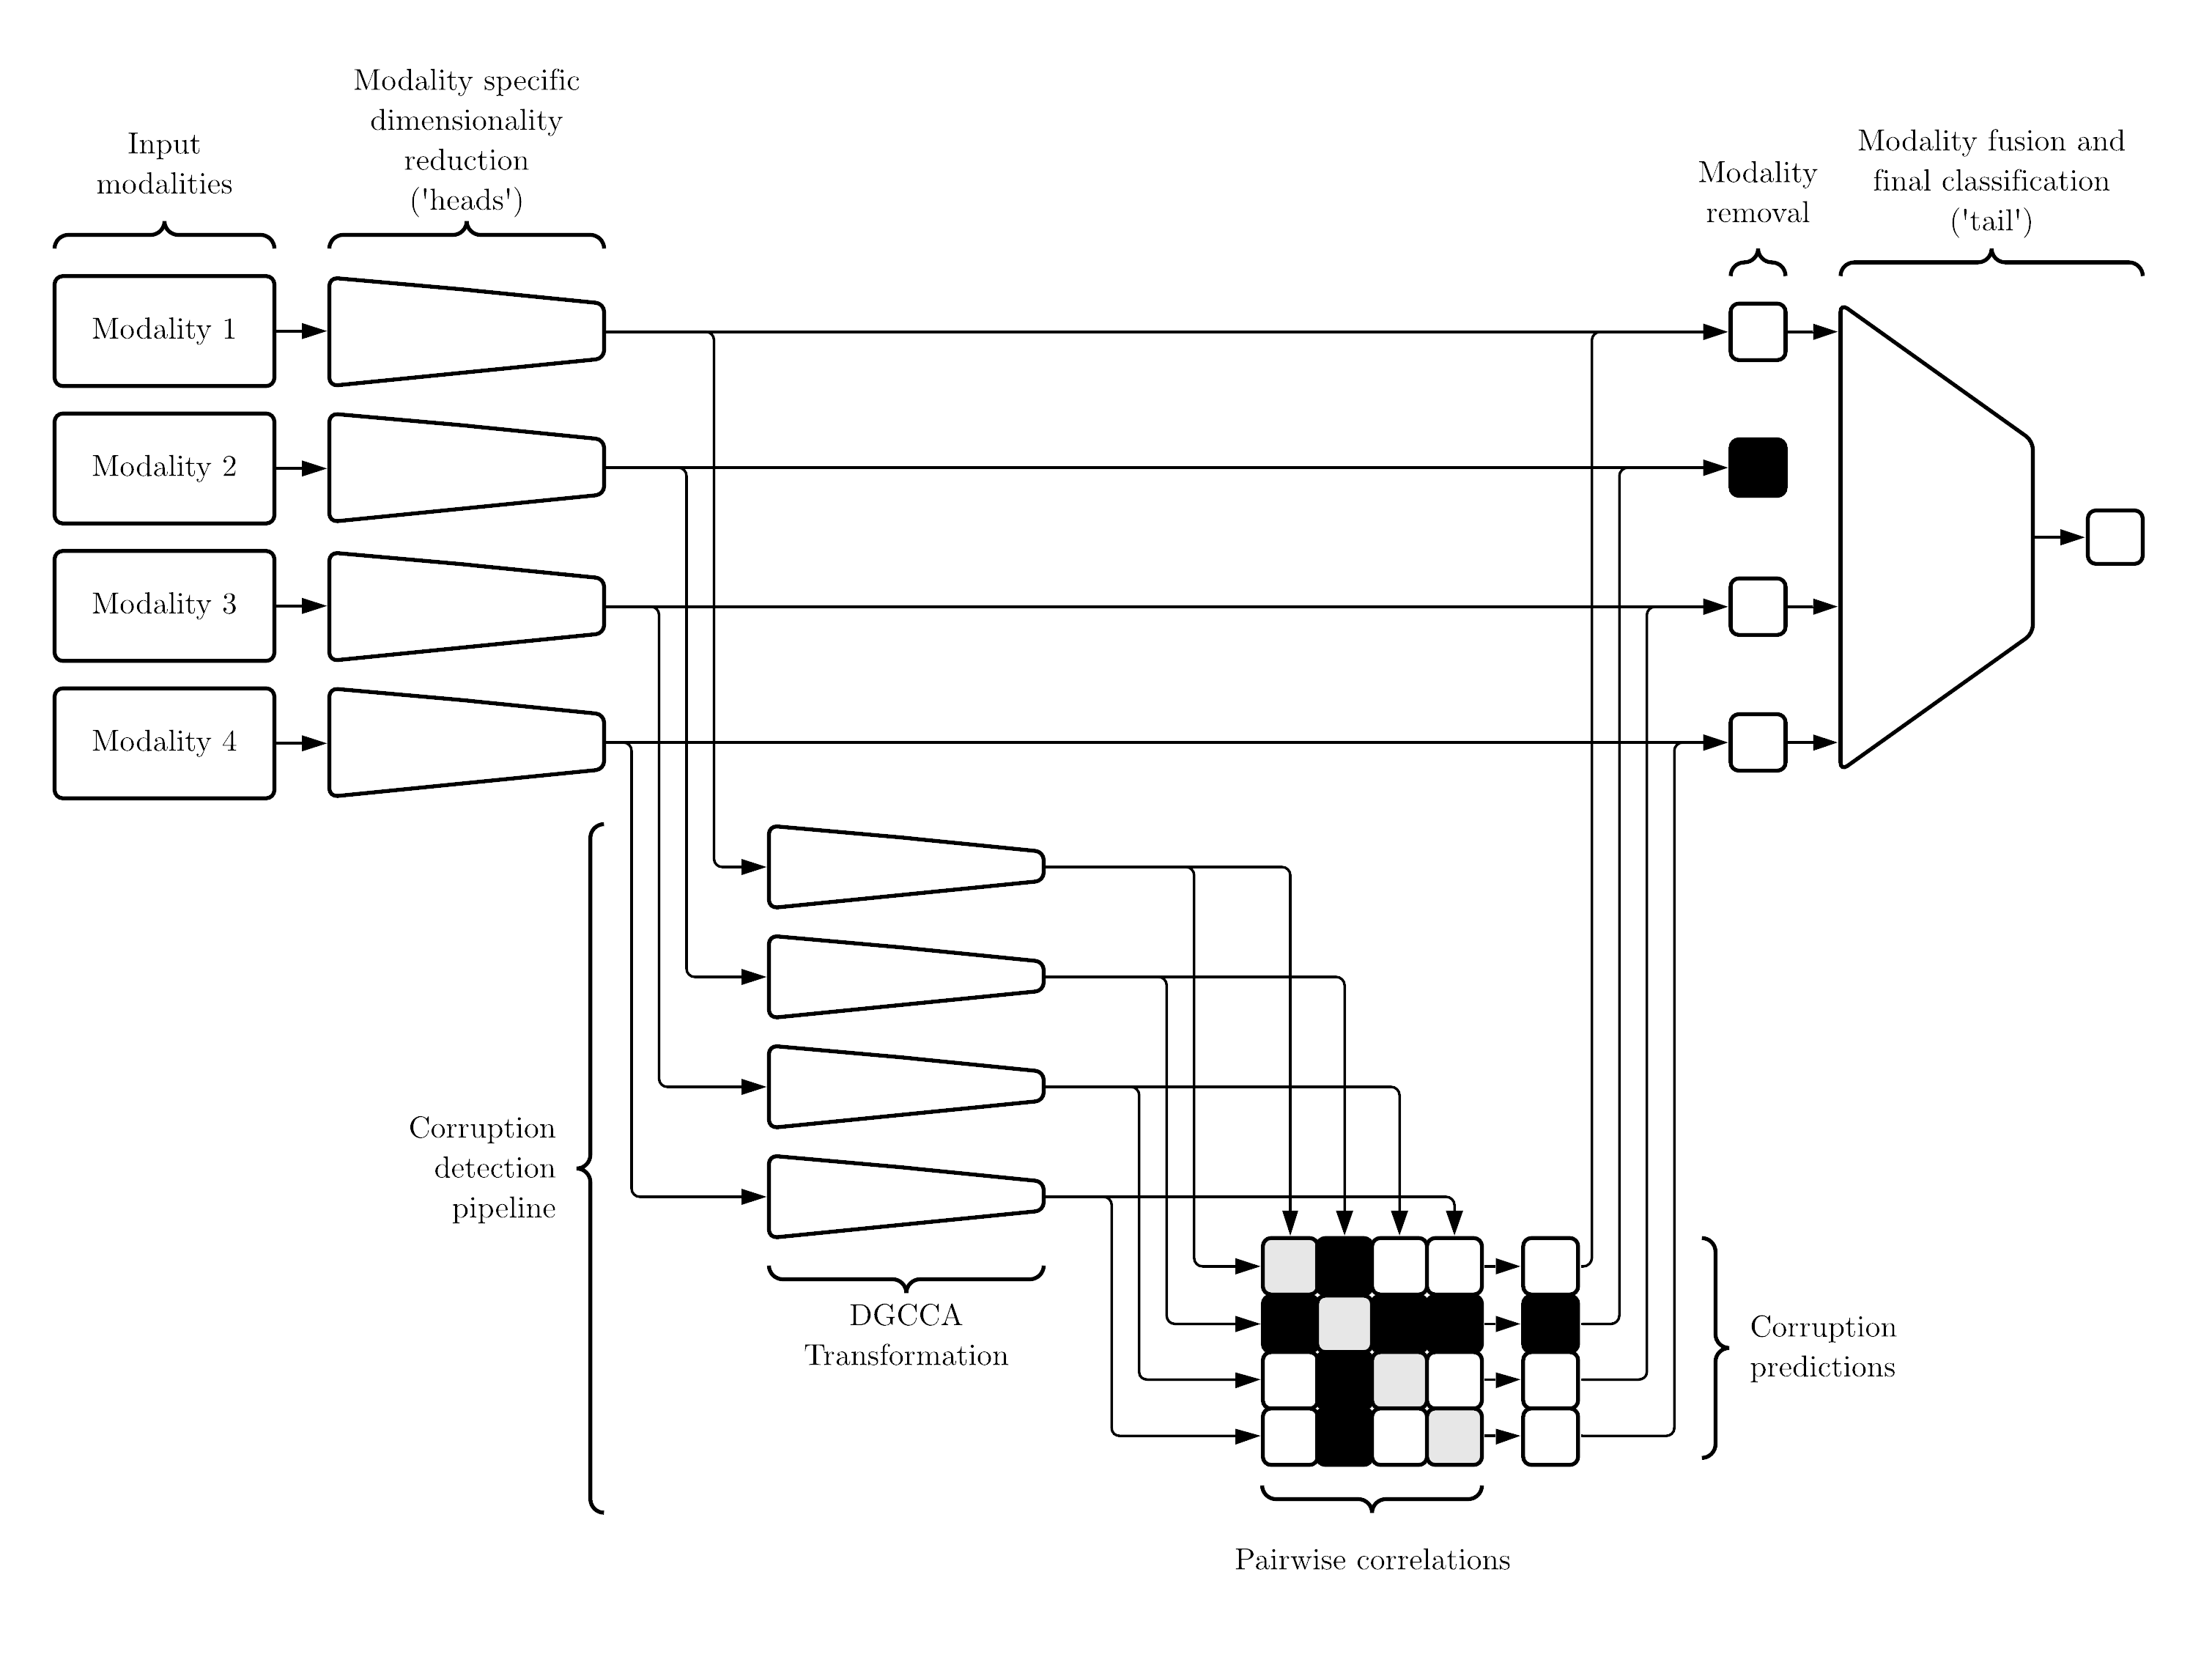
\includegraphics[width=\textwidth]{images/pipeline.png}
    \caption{Main components of the multimodal classifier and corruption detection pipeline}
    \label{fig:pipeline}
\end{figure}

2
\section{Canonical Correlation Analysis}
\subsection{Linear CCA}
Canonical Correlation Analysis \cite{CCA} is a a generalised way of analysing cross covariance matrices between two random variables. Given two random variables $\mathbf{X}=(X_1,...,X_n | X_i\in\mathbb{R}^{d_X})$ and $\mathbf{Y}=(Y_1,...,Y_n | Y_i\in\mathbb{R}^{d_Y})$, CCA learns transformations $\mathbf{u}_1\in\mathbb{R}^{d_X}$ and $\mathbf{v}_1\in\mathbb{R}^{d_Y}$ such that $$corr(\mathbf{u}_1^T\mathbf{X}, \mathbf{v}_1^T\mathbf{Y}) \textrm{ is maximised.}$$ $(\mathbf{u}_1^T\mathbf{X}, \mathbf{v}_1^T\mathbf{Y})$ are known as the first pair of canonical variables. Further canonical variables maximise correlation orthogonally to the first pair of canonical variables, with the $i^{th}$ pair of canonical variables $(\mathbf{u}_i^T\mathbf{X}, \mathbf{v}_i^T\mathbf{Y})$ maximising $$corr(\mathbf{u}_i^T\mathbf{X}, \mathbf{v}_i^T\mathbf{Y})$$ subject to $$cov(\mathbf{u}_i^T\mathbf{X}, \mathbf{u}_j^T\mathbf{X}) = cov(\mathbf{v}_i^T\mathbf{Y}, \mathbf{v}_j^T\mathbf{Y}) = 0,\thinspace  \forall \thinspace  j<i$$

In practice, CCA is carried out by performing singular value decomposition on the covariance matrix and taking the top $k$ eigenvectors. \\

The transformations learned by CCA give the basis for the anomaly detection system. When two modalities contain clean data of the type encountered during training, it is expected that their canonical variables have a high correlation. If a modality contains corrupted data which differs enough from the training distribution, the transformation will not be optimal it is expected that the correlation will be lower.\\

As discussed, CCA is limited to maximising correlations between two sets of variates using linear transformations. To use CCA efficiently with many modalities a method of learning transformations for more than two sets of variates is required.

\subsection{Generalised Canonical Correlation Analysis}
GCCA \cite{GCCA} constructs a shared representation $G$ and maximises the correlations between each set of variates and the shared representation.

\subsection{Deep Generalised Canonical Correlation Analysis}
DGCCA builds upon Deep CCA \cite{DCCA} to extend GCCA to learn nonlinear transformations. A neural network is trained for each modality to learn a nonlinear transformation to a new representation which is used for GCCA. The networks are trained by backpropagating the objective of GCCA, maximising the ability of their outputs to be correlated.\\

Benton et al. \cite{DGCCA} derive a loss function for GCCA based on pairwise correlations between modalities.\\

Using DGCCA representations of any number of modalities can be obtained, with the expectation that correlation between any two representations is high.

\section{Noise Generation}
For training and evaluation of the anomaly detector a method of adding noise to the input modalities is required. A number of different methods of noise generation are used:
\begin{itemize}
    \item Gaussian noise: Sample from the standard normal distribution for each feature in the input modality.
    \item Feature GMM: Sample from 1-D GMMs fitted to each feature of the input modality.
    \item Modality GMM: Sample from multi dimensional GMMs fitted to each modality.
    \item Full GMM: Sample from a multi dimensional GMM fitted to the entire dataset.
\end{itemize}
It is expected that each method produces more realistic and harder to detect noise than the previous, with more gmm components producing more realistic noise. Noise is added to the raw data on a per-modality basis before it is passed through the first stage of the classifier based on the signal to noise ratio specified (Figure \ref{fig:noise}), with a corrupt modality given by $corrupt = \frac{snr\times \mathbf{raw} + \mathbf{noise}}{snr + 1}$.

\begin{figure}[H]
    \centering\captionsetup{width=.8\linewidth}
    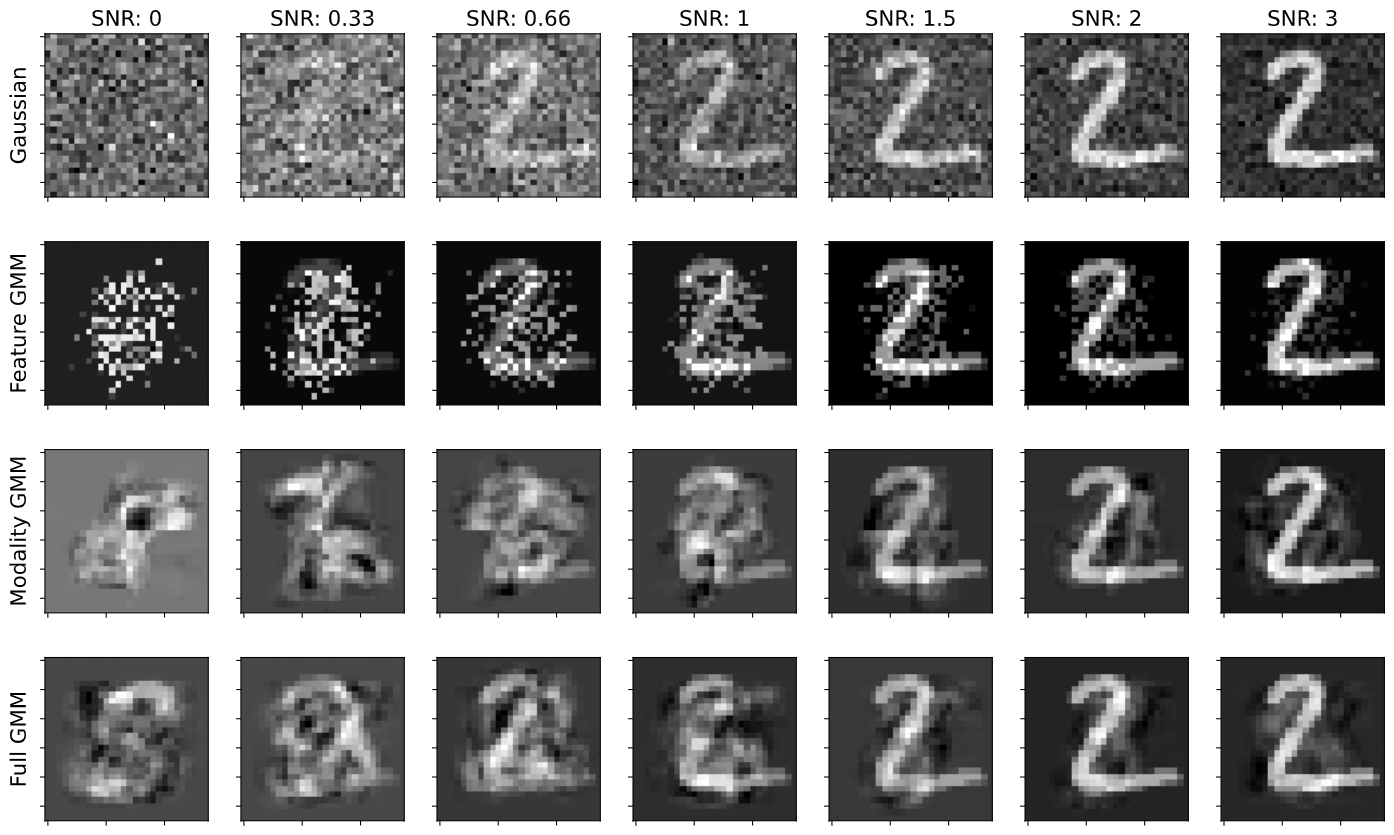
\includegraphics[width=.9\textwidth]{images/noise.png}
    \caption{An example MNIST image under varying types and strengths of noise, with all gaussian mixture models containing 5 components.}
    \label{fig:noise}
\end{figure}

\section{Corruption detection}
The general method for detecting corrupt modalities involves first looking at correlation between each of the $\frac{1}{2}(m-1)m$ possible pairs of modalities and using the information gained from each of these comparisons to infer which modalities are corrupt.

\subsection{Pairwise corruption detection}
To observe the level of correlation between two modalities we require multiple samples. We use the transformations learned by DGCCA to generate a representation of each modality. To calculate the correlation between modalities $a$ and $b$ based on $N$ samples with cca dimension $C$, we have canonical variate matrices $A, B \in \mathbb{R}^{N\times C}$ and again experiment with two different methods. 
\begin{itemize}
    \item Combined correlation, the sum of correlations over each canonical variate:
$$CombinedCorr(A, B) = \sum_{d=1}^C{corr((A_{s,d} | s=1..N), (B_{s,d} | s=1..N))}$$
    \item Flat correlation, the correlation between the flattened canonical variate matrices:
$$FlatCorr(A, B) = corr((A_{s,d} | s=1..N, d=1..C), (B_{s,d} | s=1..N, d=1..C))$$
\end{itemize}

The expectation is that these measures are high when samples are drawn from a similar distribution to the training set, but low when samples are corrupted and fall outside of it. Note that $CombinedCorr$ requires at least two samples, whilst $FlatCorr$ can be used to calculate correlation between single samples.\\

To detect whether a given pair of modalities is corrupted, we compare their correlation with a threshold learned during training. Combined correlation is calculated between cca embeddings of clean data, as well as between clean and corrupt data. The intensity of corruption used affects the distribution of corrupt correlations, and therefore the learned threshold.\\

We assume the correlations follow a normal distribution and experiment with two methods of choosing a threshold. To maximise accuracy of each pairwise anomaly detector (Figure \ref{fig:threshold_dist}), we choose the thresholds as the intersection between probability density functions of clean and corrupt modalities. To minimise the number of false negatives (Figure \ref{fig:ppf_dist}) (clean modalities erroneously classified as corrupt) we choose the thresholds as a percentile of the clean distribution.

\begin{figure}[ht]
    \captionsetup{width=.9\linewidth}
    \begin{subfigure}{.5\textwidth}
      \centering\captionsetup{width=.8\linewidth}
      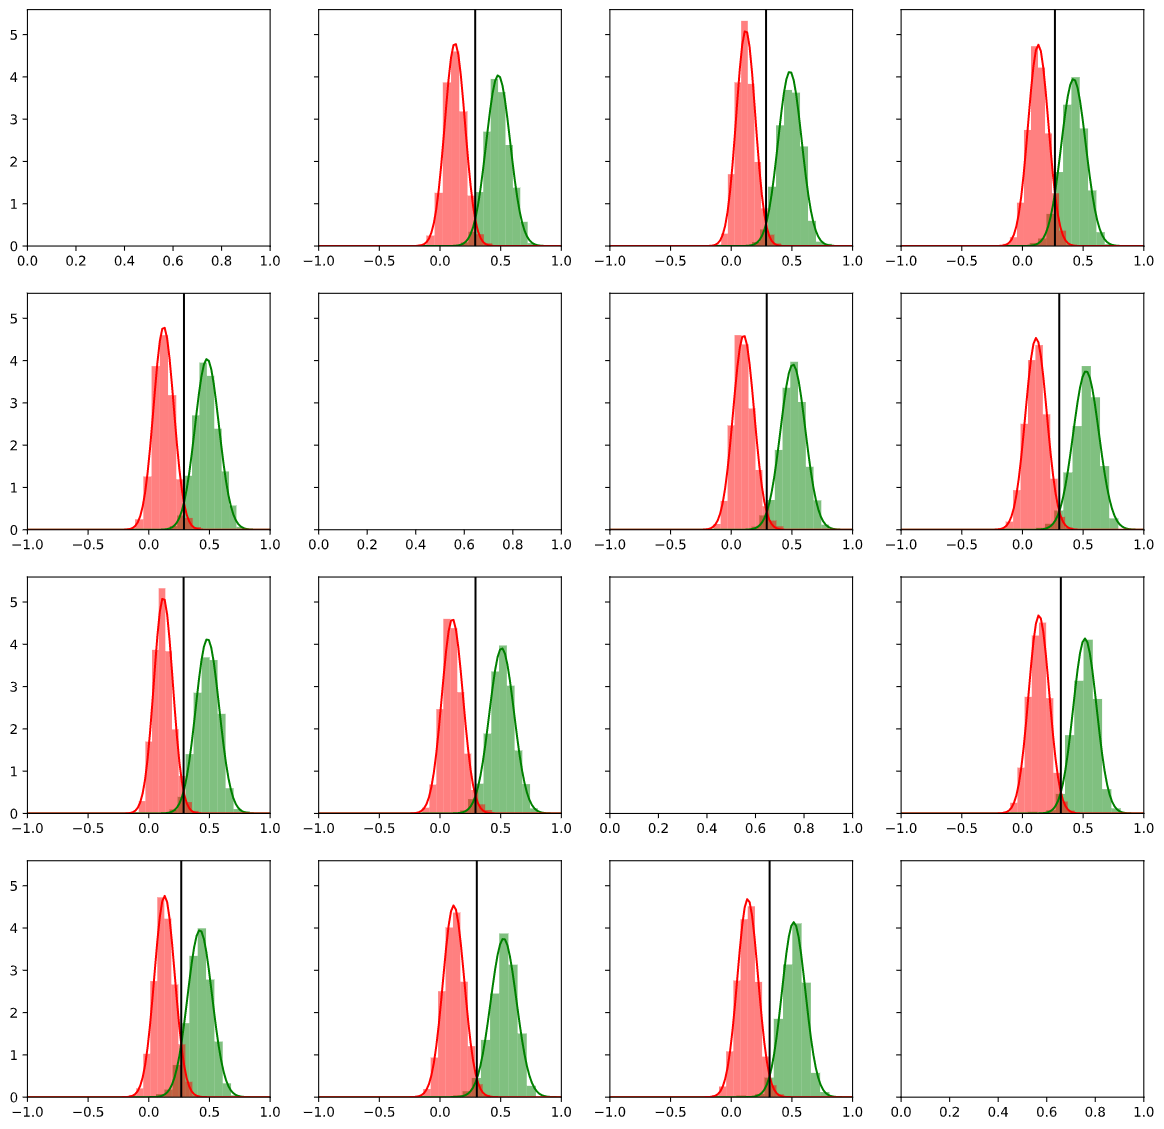
\includegraphics[width=.9\linewidth]{images/threshold_dist_clean.png}  
      \caption{Correlation thresholds using the intersection method. $P($type I error$)=0.028, P($type II error$)=0.023$}
      \label{fig:threshold_dist}
    \end{subfigure}
    \begin{subfigure}{.5\textwidth}
      \centering\captionsetup{width=.8\linewidth}
      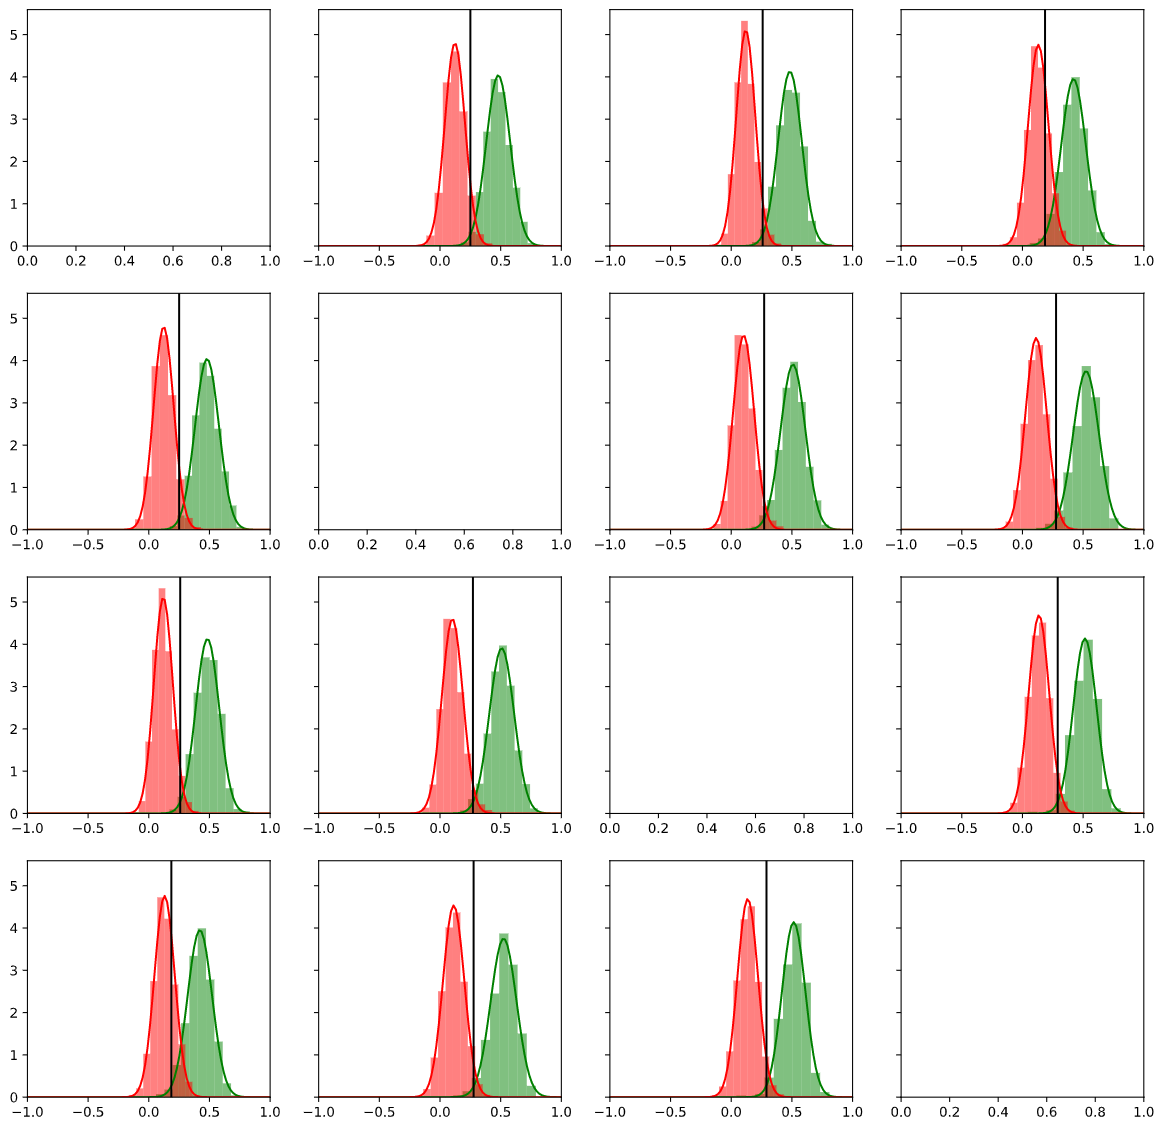
\includegraphics[width=.9\linewidth]{images/ppf_dist_clean.png}  
      \caption{Correlation thresholds using the percentile method with p-value 0.01. $P($type I error$)=0.010, P($type II error$)=0.074$}
      \label{fig:ppf_dist}
    \end{subfigure}
    \caption{Pairwise correlation distributions using two different threshold methods. Note the probability of a false negative can be chosen using the percentile method, giving a much smaller probability in Figure (b) than in Figure (a).}
    \label{fig:correlation_dist}
\end{figure}

\todo{Image of modality corruption from pairwise corruption}

\subsection{Modality corruption detection}
The pairwise corruption detection stage yields a matrix $M\in\mathbb{B}^{m\times m}$, where $M_{i,j}$ is true if both modalities are clean, and false if one or both modalities are corrupted. We expect that when modality $i$ is corrupted, all entries of the ith row and column are false. The remaining modalities are true for all entries except that of the corrupted modality. This means that when many modalities are corrupted the row corresponding to a clean modality may still contain many corrupt pairs, making classification at this stage more difficult. A number of different methods of classification have been used. Note that at least 2 modalities must be clean for any classification to be carried out, fewer clean modalities will result in all pairwise classifications being negative, so any system using pairwise correlations can detect corruption in at most $m-2$ modalities.

\begin{figure}[H]
    \centering\captionsetup{width=.8\linewidth}
    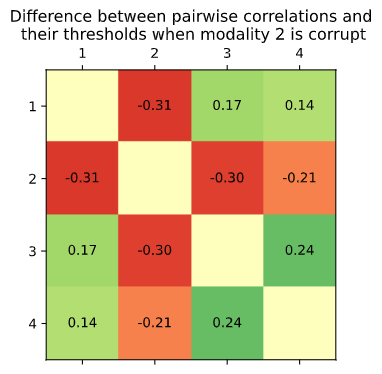
\includegraphics[width=.5\textwidth]{images/all_corrs.png}
    \caption{Relative corruption detected in modality pairs when modality 2 is corrupt in a 4 modality anomaly detector. Pairs containing modality 2 have correlations below their thresholds whilst the rest have correlations above their thresholds. The leading diagonal is ignored.}
    \label{fig:all_corrs}
\end{figure}

\subsubsection{Proportional classification}
let $k$ be the proportion of pairs that are classified as corrupt. let $k_i$ be the proportion of pairs in row $i$ that are corrupt. We expect that $k_i = 1$ when modality $i$ is corrupt, and $k_i = \frac{c}{m-1}$ otherwise. When $M$ contains both clean and corrupt pairs and pairwise corruptions are 100\% accurate $1>k>\frac{c}{m-1}$. Therefore, by measuring $k$, we can mark modality $i$ as corrupt if $k_i > k$, or clean otherwise.\\
In practice the accuracy of this method suffers when pairs are falsely classified as corrupt. If all modalities are clean, a single false negative pair classification can cause up to 2 modalities to be classified as corrupt, massively impacting accuracy.

\subsubsection{Corruption estimation}
$k$ can be calculated from the number of corrupt modalities $c$ by 
\todo{Derivation in appendix?}
$$
k = 1-\frac{(n-c)(n-c-1)}{n(n+1)}
$$
As we can calculate an estimate of $k$ directly from $M$, we can use the formula to estimate the number of corrupt modalities $c'$. If $c'$ is an integer, we can be more confident that the number of pairwise classification errors is low, otherwise we can be certain there are some errors. We can also use $c'$ to limit the number of modalities we classify as corrupt. Tests have been carried out limiting the number of corrupt modalities by rounding $c'$ to the nearer, higher, or lower integer.

\subsubsection{Delta/Probablity classification}
Rather than using the matrix $M$, we can use the difference between pairwise correlations and their trained thresholds to get a deeper view of corruption, based on the assumption that a genuinely corrupt pair will have a correlation further below their threshold than a false negative. We sum the differences across each row and mark the modality with the greatest negative value as corrupt, removing its correlations from $M$. We continue until no row has a negative total correlation. A variation uses the probability distributions learned during threshold training to estimate the probability correlation belongs to the clean and corrupt distributions. If the sum of corrupt probabilities is greater than the sum of clean probabilities, we classify a modality as corrupt, again removing its probabilities from $M$.

